\chapter{RPC \& API \& MOM}
	\section{RPC}
		\subsection{Data Conversion Problems without RPC-Middleware}
			\begin{itemize}
				\item Converting data structures into messages: Data structure as processed by programs must be flattened and reconstructed for exchange (\textbf{(de-)marshalling, (de-)serialization})
				
				\item Converting data types: Sender and receiver may be implemented in different programming
				languages that support different sets of data types or may use different representation for some data types
			\end{itemize}
			$ \Rightarrow $ Solution: Standard data representation; e.g. CORBA: CDR, Web Services: SOAP
			
		\subsection{Other Problems}
			\begin{itemize}
				\item Binding: Finding appropriate services amongst collection of services on
				various machines
				
				\item Fault Handling: Transparent handling of (communication, invocation,\ldots) errors, e.g. Network is down, Machine is busy, Duplicated requests, \ldots
			\end{itemize}
			$ \Rightarrow $ Solution: Interface definition languages (IDLs)
			
		\subsection{IDLs}
			\begin{itemize}
				\item Language to describe services in an abstract manner. Definitions are independent of the PL used to implement clients and services $ \rightarrow $ Supports interoperability btw. languages
				
				\item Code is generated to be invoked by client and code that invokes services on server that deals with all these problems – so-called stubs
			\end{itemize}
			\begin{figure}[h!]
				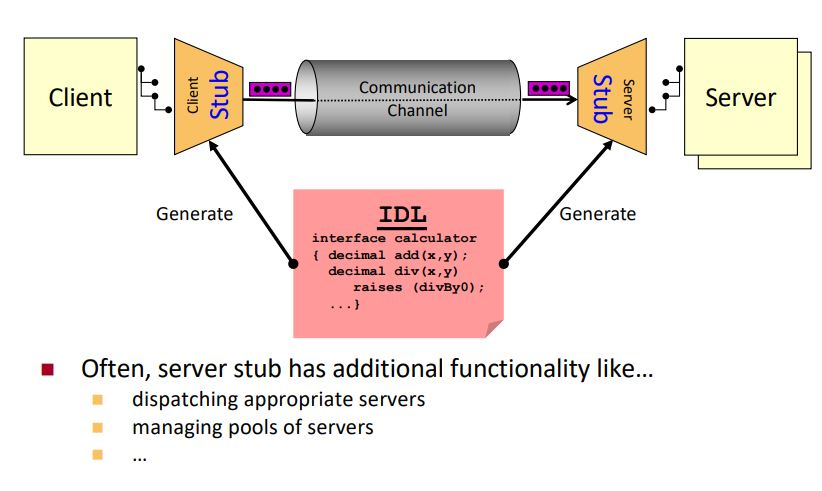
\includegraphics[scale=0.5]{res/idl-stubs.jpg}
			\end{figure}
		
	\section{API}
		API = The set of combined interfaces making the functions of a particular application available in a coherent
		manner.
		\subsection{Structure of a remote API}
			A remote API is split into two parts: The proxy on the client side and the stub on the application side.
			Communication logic is between the proxy and the stub.\\
			client programs against the	proxy and doesn’t know whether the functions used reside on its	local machine or on some remote machine $ \rightarrow $ Local/remote transparency
			
		\subsection{CORBA -- RPC for objects}
			CORBA is an Object Management Group specification for a	\textbf{C}ommon \textbf{ORB} \textbf{A}rchitecture (ORB explained later).\\
			Defines a metamodel for (distributed) objects and a corresponding IDL (CORBA IDL)\\
			Bindings of this IDL to different programming languages are	specified
			
			\subsubsection{Object Request Broker (ORB)}
			\begin{itemize}
				\item mediates remote method invocations in (remote) distributed object systems
				\item supports communication between executables implemented in different programming languages
			\end{itemize}
			\begin{figure}[h!]
				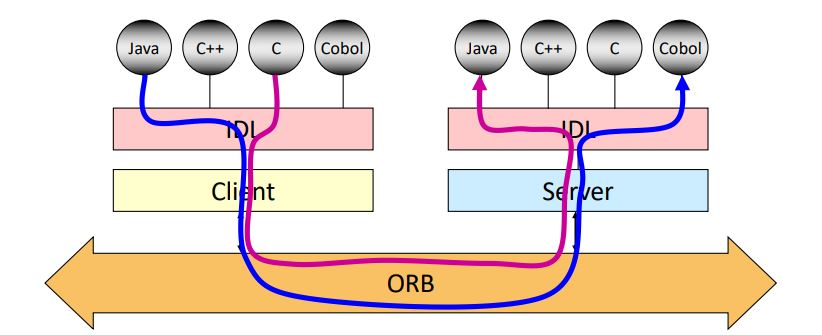
\includegraphics[scale=0.7]{res/orb.jpg}
			\end{figure}
		
		
			\subsubsection{CORBA Architecture}.
				\begin{figure}[h!]
					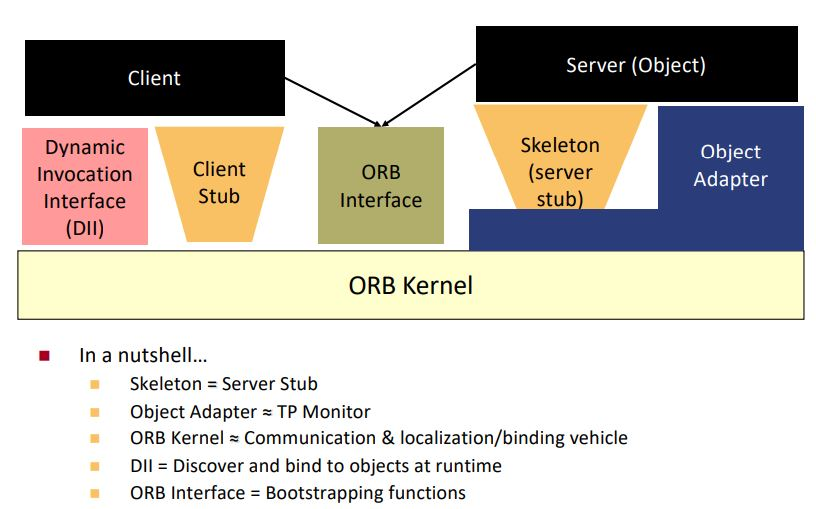
\includegraphics[scale=0.6]{res/corba-arch.jpg}
				\end{figure}
			
			\pagebreak % for layout reasons
			
			\subsubsection{ORB interoperability}
			CORBA ORBs of different vendors have to interoperate $ \Rightarrow $ GIOP (General Inter-ORB Protocol)\\
			IIOP specifies how GIOP is done over TCP\\
			Two ways of connecting ORBs: 
			\begin{enumerate}
				\item Full Bridge (Request-Level Bridge): Bilateral non-standard bridge for interoperation
				between two environments
				
				\item Half Bridge (Inline Bridge): Mapping from/to vendor specifics to IIOP
			\end{enumerate}
			Half bridges are way more common than full bridges.
			
			
			
	\section{MOM (Message Buses)}
		\subsection{Basics}
			Distributed functions can use messaging to communicate and transfer data. But sending data to another computer is a lot more complicated and requires data to be copied from one computer to another $ \rightarrow $ data has to be serializable\\
			When connecting multiple computer systems via remote communication, these systems likely use different languages, technologies and platforms. Messaging system can be a universal translator between
			applications, allow them to communicate through a common messaging paradigm.\\
			\textbf{This is called a message bus or MOM}
			
			
			
		\subsection{Advantages}
			\subsubsection{Asynchronous Communication}
				The sender does not have to wait for the receiver to receive and process the message
			\subsubsection{Variable Timing}
				the	sender can batch requests to the receiver at its own pace, and the receiver can consume them  at its own (probably different) pace
			\subsubsection{Avoid Throttling}
				Too many RPC calls at a time can overload the receiver and even cause it to crash. Asynchronous communication enables the receiver to control the rate at which it consumes requests. Effect on thee caller is minimal because it does not have to wait for the receiver.
			\subsubsection{Reliability}
				Messaging provides reliable delivery through the
				\begin{itemize}
					\item Store and forward
					\item guaranteed delivery
				\end{itemize}
				approaches.
				
			
		\subsection{Disadvantage: Complex Programming Model}
			ogic is split up into a number of event handlers that respond to incoming messages. Such a system is more complex and harder to develop and debug.\\
			Moreover, Transaction model is most often compensation based, more complex than ACID and 2PC.
			
			\pagebreak % Aus Layout-Gründen
			
			
		\subsection{Message Queuing -- MQM (Message Queue Manager)}
				 Provides environment for queuing applications. 
				 \begin{itemize}
				 	\item provides reliable storage for queued messages
				 	\item manages concurrent access to data
				 	\item ensures security and authorization
				 	\item provides special queuing functions (like triggering)
				 \end{itemize}
				 Applications connect to exactly one MQM which is then called the \textit{local MQM} and then use the Message Queuing interface (MQI).
				 \begin{figure}[h!]
				 	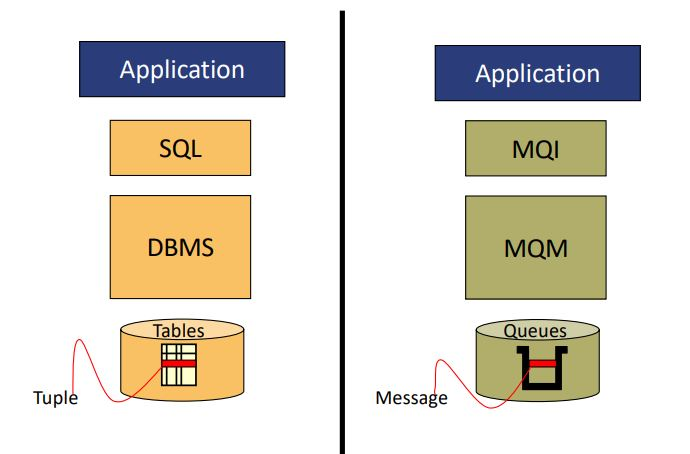
\includegraphics[scale=0.4]{res/mqm-analogy-dbs.jpg}
				 	\caption{Analogy for people familiar with Databases}
				 \end{figure}
			 
			 \subsubsection{Delivering Remote Messages -- The Mover}
			 \begin{itemize}
			 	\item processes messages in a transmission queue jointly with its partner mover at the other end of the channel, thus ensuring reliable transmission to	remote MQM\\
			 	$ \Rightarrow $ realization of the guaranteed delivery approach
			 	
			 	\item  Failures are tolerated: The only effect of a channel failure is a delay of the message transmission until channel becomes available again ($ \approx $ 2PC protocol)
			 \end{itemize}
		 
		 
		\subsection{Message Queuing -- MQI (Message Queuing Interface)}
			Target of communication is queue, not program.\\
			Two important concepts:
			\begin{enumerate}
				\item \textbf{send-and-forget}: Program simply puts message to queue and continues processing
				\item \textbf{store-and-forward} (if queue is remote): local MQM ensures delivery to remote queue

			\end{enumerate}
			\begin{figure}[h!]
				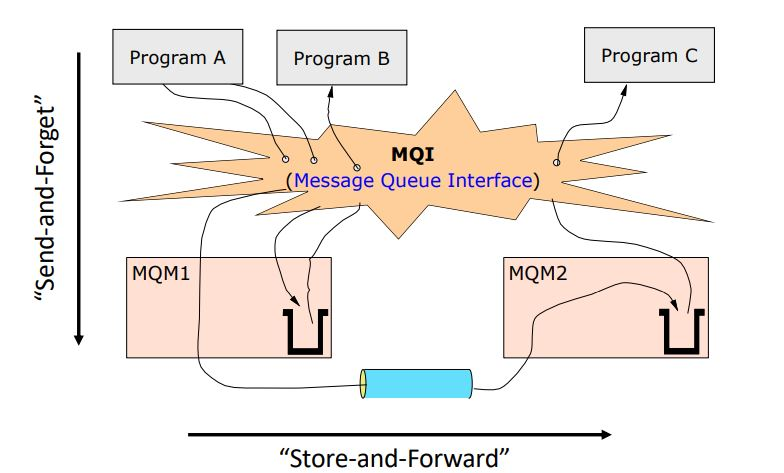
\includegraphics[scale=0.5]{res/mqi.jpg}
				\caption{The MQI}
			\end{figure}
		
		\pagebreak % for layout reasons
		
			\subsubsection{MQI vocabulary}
				\begin{itemize}
					\item \textbf{MQCONN}: Connects a program to a MQM; A particular MQM can be specified by name
					
					\item \textbf{MQDISC}: Tells the MQM to release resources required for supporting the program; All open queues are implicitly closed
					
					\item \textbf{MQOPEN}: Gives a program access to a particular queue (a program can have concurrent access to multiple queues)
					
					\item \textbf{MQCLOSE}: Tells the MQM to release the resources needed to support the programs operations on the associated queue
					
					\item \textbf{MQINQ}: Retrieves attributes of a particular queue and the MQM connected to it (example: Number of messages in queue, number of programs which opened the queue, \ldots)
					
					\item \textbf{MQSET}: Alters the current values of attributes of an object (example: Number messages required in queue before triggering occurs)
					
					\item \textbf{MQPUT}: Puts message in a queue (local or remote)
					
					\item \textbf{MQGET}: Retrieve a message from a specified queue (FIFO or selectively); Specified queue must be local!

				\end{itemize}
				(More in the slides\ldots)
				
		
		\subsection{Principles}
			\subsubsection{PubSub (PublishSubscribe)}
				A sender publishes a message to a \textit{topic}; Zero or more \textit{subscribers} to that topic get this message
				\begin{figure}[h!]
					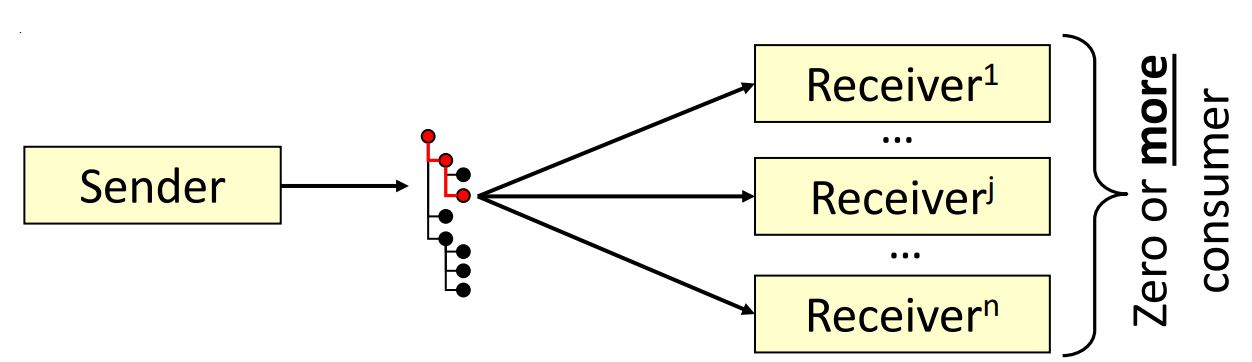
\includegraphics[scale=0.25]{res/pubsub.jpg}
				\end{figure}
			
				\textbf{Topics} can have 0 or more topics as children; topic without parent is called \textit{root topic}. The hierarchy consisting of a root topic and all its descendants is called a \textit{topic tree}. A subscriber of a topic automatically subscribes to all of its children.
				
			\subsubsection{Loose coupling}
				Reduce number of assumptions two parties make about each other when they exchange information $ \rightarrow $ more tolerance to changes at a partner's side\\
				But more assumptions increase efficiency $ \rightarrow $ in high-performance environments, coupling is tight. Loose Coupling also affords	
				\begin{itemize}
					\item platform
					\item time
					\item reference
					\item format
				\end{itemize}
				autonomy.
			
			
			
			
			
			
			
			
			
			
			
			
			